% Copyright (c)  2005-2010 EDF-EADS-PHIMECA.
% Permission is granted to copy, distribute and/or modify this document
% under the terms of the GNU Free Documentation License, Version 1.2
% or any later version published by the Free Software Foundation;
% with no Invariant Sections, no Front-Cover Texts, and no Back-Cover
% Texts.  A copy of the license is included in the section entitled "GNU
% Free Documentation License".
\renewcommand{\etapemethodo}{Resp. Surf.}
\renewcommand{\nomfichier}{docref_SurfRep_Enum}
\renewcommand{\titrefiche}{Strategies for enumerating the polynomial chaos basis}

\newcommand{\mathA}{\mathcal{A}}
\renewcommand{\idx}{\underline{\alpha}}
\newcommand{\NM}{\mathbb{N}^{n_X}}

\Header

\MathematicalDescription{
\underline{\textbf{Goal}} \vspace{4mm}

The polynomial chaos (PC) expansion allows one to obtain an explicit representation of the random response $\underline{Y}$ of the model under consideration, see~\otref{docref_SurfRep_PCBasis}{PC basis}. More precisely, the response is cast as a converging series featuring orthonormal polynomials. For computational purpose, it is necessary though to retain a finite number of terms by truncating the expansion. First of all, a specific strategy for enumerating the infinite PC series has to be defined. This is the scope of the current section.\\

\underline{\textbf{Enumerating strategies}} \vspace{4mm}

Given an input random vector $\bs{X}$ with prescribed probability density function (PDF) $f_{\bs{X}}(\bs{x})$, it is possible to build up a \emph{polynomial chaos} (PC) basis $\{\psi_{\idx},\idx \in \NM\}$ \otref{docref_SurfRep_PCBasis}{Polynomial chaos basis}. Of interest is the definition of enumeration strategies for exploring this basis, i.e. of suitable \emph{enumeration functions} $\tau$ from $\Nset$ to $\NM$, which creates a one-to-one mapping between an integer $j$ and a multi-index $\idx$. 

\paragraph*{Linear enumeration strategy \\ \\}

Let us first define the \emph{total degree} of any multi-index $\idx$ in $\NM$ by $\sum_{i=1}^{n_X} \alpha_i$. A natural choice to sort the PC basis (i.e. the multi-indices $\idx$) is the lexicographical order with a constraint of increasing total degree. Mathematically speaking, a bijective enumeration function $\tau$ is defined by:
\begin{equation}
 \begin{array}{llcl}
 \tau \, : & \Nset & \longrightarrow & \NM \\
           &  j & \longmapsto & \{\alpha_1,\dots, \alpha_M\} \, \equiv \, \{\tau_1(j),\dots,\tau_M(j)\} \\
\end{array}
 %\forall j \; \geq \; 1 \quad \, , \quad \, 
\end{equation}
such that:
\begin{equation}
\tau(0) \, \, = \, \, \{0,\dots,0\}
\end{equation}
and
\begin{equation}
\forall 1 \leq j<k  \quad \, , \quad \, \left\{
\begin{array}{l}
\displaystyle{\sum_{i=1}^{n_X} \tau_i(j) \, < \,  \sum_{i=1}^{n_X} \tau_i(k)  }  \\
\\
\mbox{ or} \\
\\
\displaystyle{\exists \; m \; \in \; \{1,\dots,n_X\} \; : \; \left( \; \forall \; i \; \leq \; m \; \; , \; \; \tau_i(j) \, = \, \tau_i(k) \; \right) \, \, \, \mbox{ and } \, \, \, \left( \; \tau_m(j) \, < \, \tau_m(k) \; \right)} \\
\end{array}
\right.
\end{equation}

%\clearpage

Such an enumeration strategy is illustrated in a two-dimensional case (i.e. $n_X=2$) in the figure below:

\begin{center}		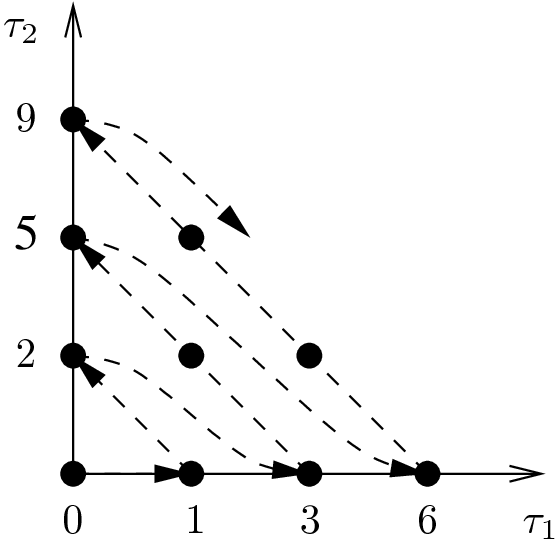
\includegraphics[width = 6.5cm]{enumerate.png} \end{center} 

This corresponds to the following enumeration of the multi-indices:

\begin{center}		
\begin{tabular}{cc}
\hline
$j$ & $\idx \, = \, \{\alpha_1,\alpha_2\} $\\
\hline
$0$ & $\{0,0\}$ \\
$1$ & $\{0,1\}$ \\
$2$ & $\{1,0\}$ \\
$3$ & $\{2,0\}$ \\
$4$ &$ \{1,1\}$\\
$5$ & $\{0,2\}$ \\
$6$ & $\{3,0\}$ \\
$7$ & $\{2,1\}$ \\
$8$ & $\{1,2\}$ \\
$9$ & $\{0,3\}$ \\
\hline
\end{tabular}
\end{center} 

\paragraph*{Hyperbolic enumeration strategy \\ \\}
The \emph{hyperbolic} truncation strategy is inspired by the so-called \emph{sparsity-of-effects principle}, which states that most models are principally governed by main effects and low-order interactions. Accordingly, one wishes to define an enumeration strategy which first selects those multi-indices related to main effects, i.e. with a reasonably small number of nonzero components, prior to selecting those associated with higher-order interactions. \\

For any real number $q$ in $(0,1]$, one defines the $q$-\emph{hyperbolic norm} (or $q$-\emph{norm} for short) of a multi-index $\idx$ by:
\begin{equation}
  \|\idx\|_{q} \, \, = \, \, \left(\sum_{i=1}^{n_X} \; \alpha^q \right)^{1/q}
\end{equation}
Strictly speaking, $\|\cdot\|_q$ is not properly a norm but rather a \emph{quasi-norm} since it does not satisfy the triangular inequality. However this abuse of language will be used in the following. Note that the case $q=1$ corresponds to the defintion of the total degree.  \\

Let $\lambda$ be a real positive number. One defines the set of multi-indices with $q$-norm not greater than $\lambda$ as follows:
\begin{equation} \label{eq_q_set}
  \mathcal{A}_{\lambda} \, \, = \, \, \{\idx \in \NM \, : \, \|\idx\|_q \, \leq \lambda \}
\end{equation}
Moreover, one defines the \emph{front} of $\mathcal{A}_{\lambda}$ by:
\begin{equation}
  \partial \mathcal{A}_{\lambda} \, \, = \, \, \left\{\idx \in \mathcal{A}_{\lambda} \, : \, \exists \; i \; \in \; \{1,\dots,n_X\} \, , \, \, \idx \, + \, \bs{e_i} \, \notin \, \mathcal{A}_{\lambda} \right\}
\end{equation}
where $\bs{e_i}$ is a multi-index with a unit $i$-entry and zero $k$-entries, $k\neq i$.  \\
% \begin{equation}
%   \bs{e_i} \, \, = \, \, \{\underrel{0,\dots,0}{(i-1)\mbox{ times}}, 1,\underrel{0,\dots,0}{(M-i) \mbox{ times}} \}
% \end{equation}

The idea consists in exploring the space $\NM$ by progressively increasing the $q$-norm of its elements. In this purpose, one wants to construct an enumeration function that relies upon (1) the bijection $\tau$ defined in the previous paragraph and (2) an appropriate increasing sequence $(\lambda_n)_{\Nset}$ that tends to infinity. Such a sequence can be used to define a specific partition of $\NM$ into \textit{stratas} $(\Delta_n)_{\Nset}$. Precisely, the enumeration of the multi-indices is achieved by sorting the elements of $\Delta_n$ in ascending order of the $q$-norm, and then by sorting the possible elements having the same $q$-norm using the bijection $\tau$. Several examples of partition are given in the sequel. \\

\textit{Partition based on the total degree. }  We can simply define the sequence $(\lambda_n)_{\Nset}$ as the set of natural integers $\Nset$. Thus we build up a sequence $(\Delta_n)_{\Nset}$ of stratas as follows:
\begin{equation}
  \left\{
\begin{array}{l}
\Delta_0 \, \, = \, \, \{\bs{0}\} \\
\forall \; n  \geq  1 \, \, , \, \, \Delta_n \, \, = \, \, \mathcal{A}_{n} \; \setminus \; \mathcal{A}_{n-1}  \, \, = \, \, 
 \{\idx \in \NM \, : \, n - 1 \, < \, \|\idx\|_q \, \leq n \}      \\
\end{array}
\right.
\end{equation}
The progressive exploration of $\NM$ is depicted in the two-dimensional case for various values of the parameter $q$:
\begin{center}	 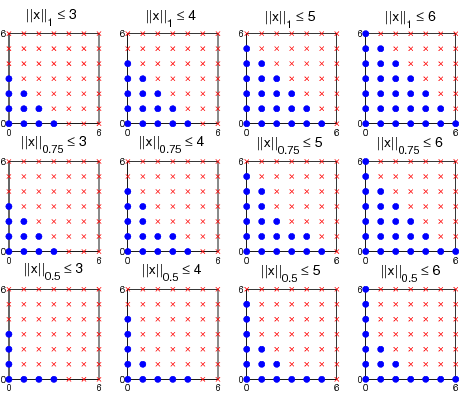
\includegraphics[width = 10cm]{qnorms_2D.png} \end{center} 

As expected, the hyperbolic norms penalize the indices associated with high-order interactions all the more since $q$ is low. Note that setting $q$ equal to 1 corresponds to the usual \emph{linear} enumeration strategy. Then the retained polynomials are located under a straight line, hence the label \emph{linear enumeration strategy}. In contrast, when $q < 1$, the retained basis polynomials are located under an hyperbola, hence the name \emph{hyperbolic enumeration strategy}. \\

\textit{Partition based on disjoint fronts. } Instead of considering the sequence of natural integers, we define the sequence $(\lambda_n)_{\Nset}$ recursively by:
\begin{equation}
  \left\{
\begin{array}{l}
\lambda_0 \, \, = \, \, 0 \\
\forall \; n  \geq  1 \, \, , \, \, \lambda_n \, \, = \, \, 
\inf_{\lambda \in \mathbb{R}^+} \; \left\{ \lambda \geq \lambda_{n-1} \, \, \mbox{ and } \, \,\partial \mathcal{A}_{\lambda} \, \cap \, \partial \mathcal{A}_{\lambda_{n-1}} \, = \, \emptyset \right\}
\end{array}
\right.
\end{equation}
In other words, $\lambda_n$ is the infimum of the real numbers $\lambda$ for which the new front contains only element which do not belong to the former one. Hence the sequence of stratas:
\begin{equation}
  \left\{
\begin{array}{l}
\Delta_0 \, \, = \, \, \{\bs{0}\} \\
\forall \; n  \geq  1 \, \, , \, \, \Delta_n \, \, = \, \, \mathcal{A}_{\lambda_n} \; \setminus \; \mathcal{A}_{\lambda_{n-1}} \\
\end{array}
\right.
\end{equation}
Note that this partition of $\NM$ is finer than the one based on total degrees, since the cardinality of the stratas is smaller.

\paragraph*{Anisotropic hyperbolic enumeration strategy \\ \\}

One might also consider enumeration strategies based on an \emph{anisotropic} hyperbolic norm defined by:
\begin{equation} 
  \|\idx\|_{\bs{w},q} \, \, = \, \, \left(\sum_{i=1}^{n_X} \; w_i\; \alpha^q \right)^{1/q}
\end{equation}
where the $w_i$'s are real positive numbers. This would lead to first select the basis polynomials depending on a specific subset of input variables. \\

In this setup, it is also possible to explore the space $\NM$ of the multi-indices by partitioning it according to one of the two schemes outlined in the previous paragraph (it is only necessary to replace the isotropic $q$-norm in Eq.(\ref{eq_q_set}) with the $(\bs{w},q)$-anisotropic one). \\

We may also build up an alternative partition related to the \emph{partial degree} of the most important variable, i.e. the one associated to the \emph{smallest} weight $w_i$. Then the sequence $(\lambda_n)_{\Nset}$ is equal to $\Nset$ and the sets $\mathcal{A}_{\lambda}$ are defined by:
\begin{equation} 
  \mathcal{A}_{\lambda} \, \, = \, \, \{\idx \in \NM \, : \, \alpha_{i^*} \, \leq \lambda \} \quad \quad , \quad \quad i^* \, \, = \, \, \mbox{arg} \min \left\{w_i \; , \; 1\leq i \leq n_X \right\} 
\end{equation}
If stratas with larger cardinalities are of interest, one may rather consider the partial degree of the least significant variable, i.e. the one associated with the \emph{greatest} weight $w_i$. To this end, the index $i^*$ in the previous formula has to be defined by:
\begin{equation} 
   i^* \, \, = \, \, \mbox{arg} \max \left\{w_i \; , \; 1\leq i \leq n_X \right\} 
\end{equation}




}

{
  --
}

\Methodology{
Within the global methodology, the polynomial chaos expansion of the model under consideration is built up prior to tackling the step C: ``Uncertainty propagation''. Then the various uncertainty propagation techniques may be applied at a negligible computational cost. The method requires to have fulfilled the two following steps:
\begin{itemize}
  \item step A1: identify of an input vector $\vect{X}$ of sources of uncertainties and an output variable of interest $\underline{Y} = h(\underline{X})$;
  \item step B: identify one of the proposed techniques to estimate a probabilistic model of the input vector $\vect{X}$.
  \end{itemize}
}
{
The hyperbolic enumeration strategy has been inspired by the following work:
\begin{itemize}
  \item G. Blatman, 2009, ``Adaptive sparse polynomial chaos expansions for uncertainty propagation and sensitivity analysis'', PhD thesis, Clermont Universit\'e.
  \end{itemize}
}


